\section{Additional}\label{Additional}


From table \ref{table:classification_results} it can be validated that the best results are obtained from the Random Forest algorithm. The second best and which allow us to have a visual representation of the decision tree to classify the events is obtained from the J.48 algorithm. In the following lines we outline the trees obtained from the J.48 algorithm from both datasets, binary and multiclass. Not all branches in the tress will match to what is expected in the wild, recall, J.48 was close to the best results, nevertheless was not the best algorithm for classification. There are certain branches from the decision trees derived from J.48 algorithm that closely match what is expected in the wild. The tree obtained from J.48 algorithm is illustrated in figure \ref{image:binary_classification_tree}.

\begin{figure}[h]
	\centering
	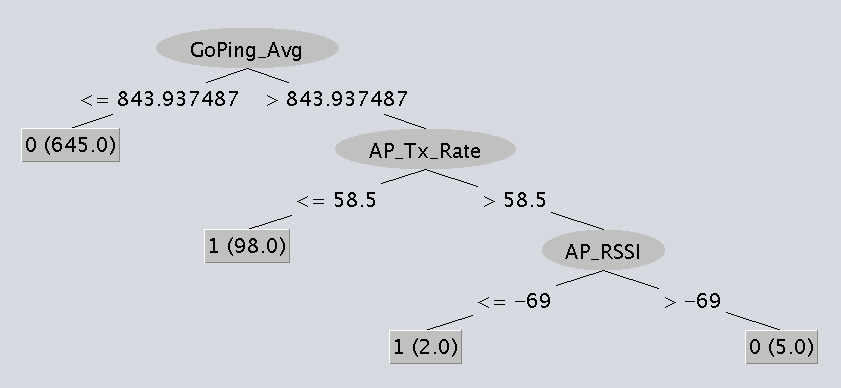
\includegraphics[width=7cm]{Classification_Trees/Binary_J_48_Tree}
	\caption{Classification Tree - Binary Dataset}
	\label{image:binary_classification_tree}
\end{figure}

\begin{figure*}[b]
	\centering
	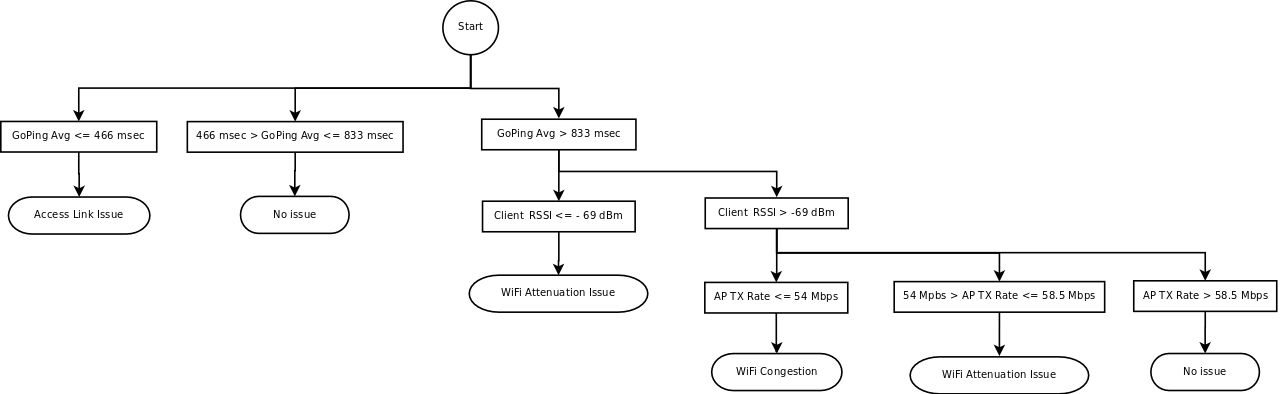
\includegraphics[width=17cm]{Classification_Trees/Multiclass_J_48_Tree}
	\caption{Classification Tree - Multiclass Dataset}
	\label{image:multiclass_classification_tree}
\end{figure*}

The tree depicts behaviors expected on Wireless impairments conditions. The first level of the three evaluates if the Avg RTT is greater than ~843 msec. The first level covers an expected behavior in which an increase in RTT can denote a complication in the Home WiFi. The second level adds more certainty by evaluating the Tx Rate of AP. If the Tx Rate of the AP falls under 58.5 Mbps the event is marked as a WiFi Issue. As a third level and in case AP Tx Rate is higher than 58.5 Mbps, the AP RSSI signal is evaluated. With an RSSI value smaller than -69 dBm the wireless condition can denote a potential attenuation issue. As in this dataset we the classification per issue is not implemented, the event is marked as WiFi issue. Still the values of the evaluated metrics follow a pattern in which a WiFi issue can be found. In summary we consider the resultant tree as accurate given the metrics and values detailed in its breakdown. The next step in our analysis was the multiclass dataset. As described before, the multiclass dataset uniquely labels each of the different events. The goal is to classify in more detail the kind of event being experienced. The resultant tree from the J.48 algorithm on the multiclass data set is detailed in figure \ref{image:multiclass_classification_tree}. The figure has been derived from the default output of Weka software in order to make the tree more readable. One of the branches which depicts an expected behavior is branch 3. The values for the two metrics enclosed in this branch illustrate what can be expected from a WiFi attenuation issue. The first level evaluates if the Avg RTT goes above ~833 msec. High RTT can denote a network issue. The next level, evaluates Client RSSI metric, one of the metrics that captures the best the attenuation and which is associated to WiFi performance. Attenuation in this scenario can be caused due to an obstacle being placed between AP and Wireless client or wireless client moving away from the AP. The decision tree captures this behavior by setting a lower bound of -69 dBm for RSSI. If the RSSI goes below this threshold the event is marked as a attenuation. Branch number 4 captures the potential case of WiFi congestion. In this branch Client RSSI is greater than -69 dBm, meaning that potentially no obstacle has been placed between AP and Wireless client or Wireless client moving away from AP. Even with a -69 dBm value there is a decrease in AP TX Rate. This behavior can be caused by congestion, AP is experiencing congestion and has the need to decrease TX Rate even with strong RSSI. These two branches are the ones in which values match an expected behavior of a Wifi issue in the wild. Still, the best classification results have been obtained with Random Forest and we forecast to use it as the algorithm for further development of our tool.


% By running these test we have validated that the amount of attribute defined helps us to properly classify the algorithms.
\newpage


